\chapter{Results}
\label{chap:results}

\section{Frontend showcase}
\label{sec:frontend-showcase}

This section showcases the resulting frontend application, which serves as the primary interface for the Roskilde Festival safety team to access and analyze crowd dynamics data. The interface is designed to be intuitive, presenting complex data through interactive charts and maps. The following figures illustrate the key features and functionalities of the application. Note that data shown from June 30th to July 2nd corresponds to the Eos stage, while data from July 3rd onwards corresponds to the Arena stage.

\begin{figure}[ht]
  \centering
  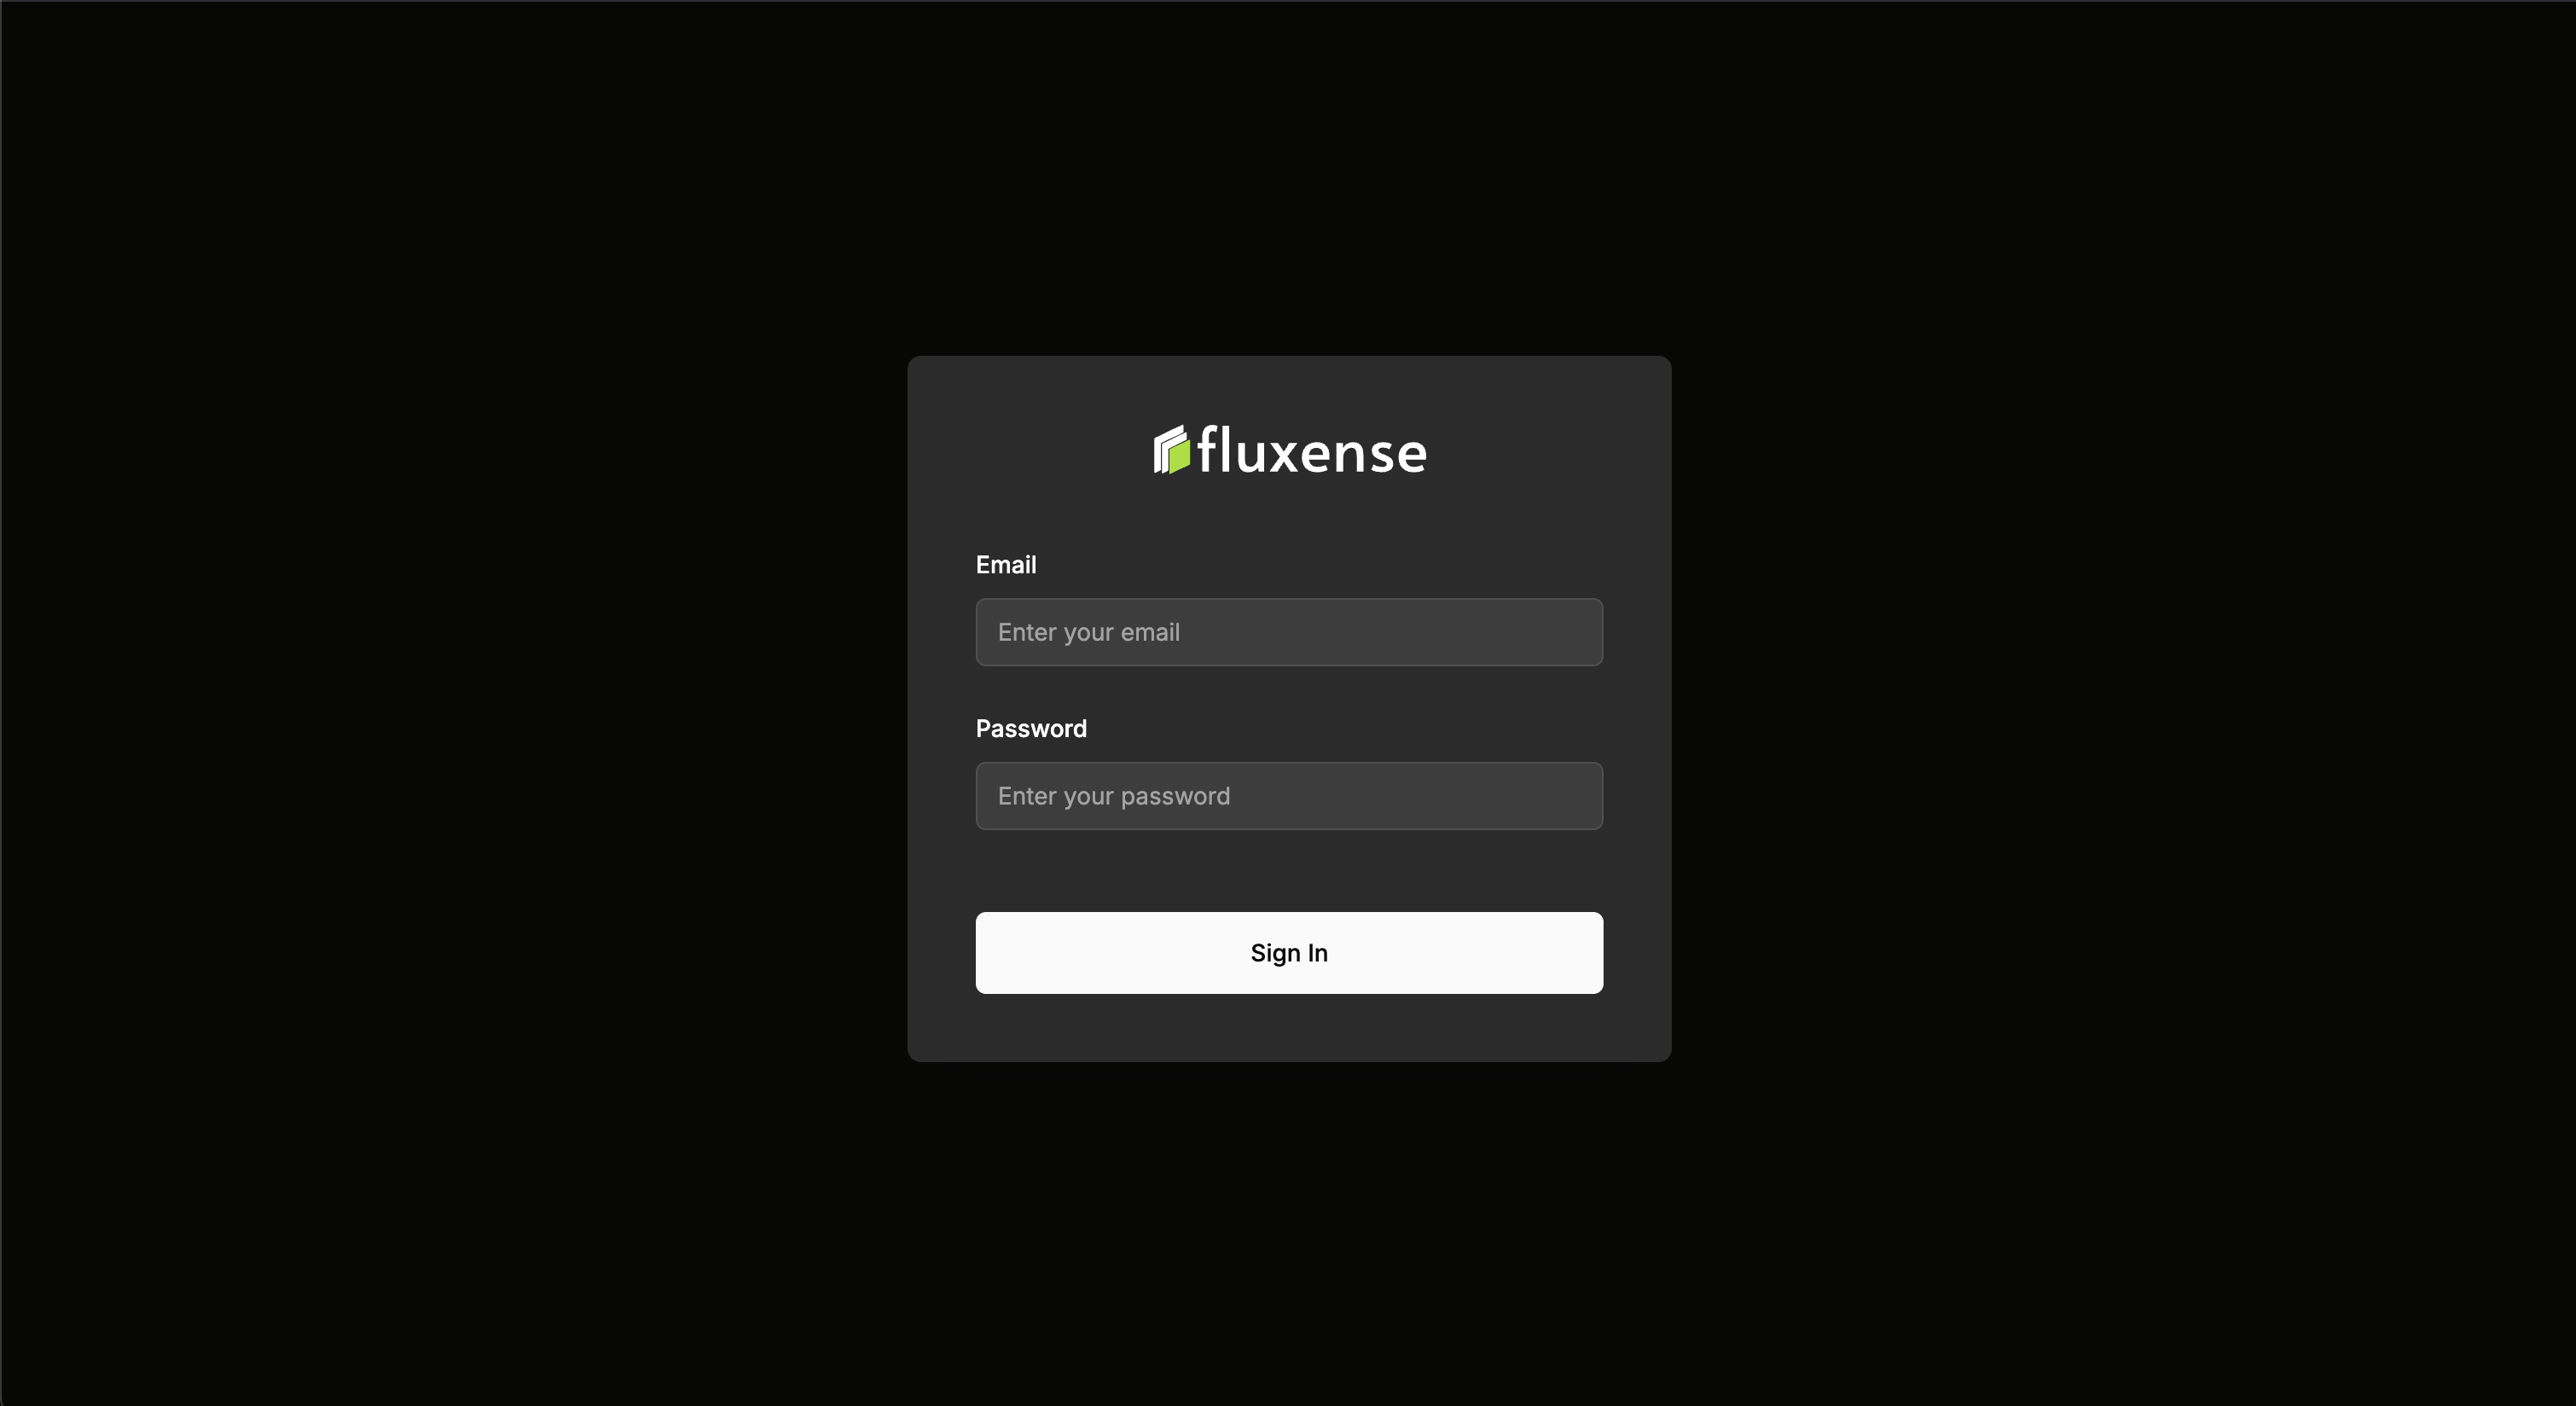
\includegraphics[width=\textwidth]{Pictures/Misc/Frontend/login.png}
  \caption{The application login screen, ensuring secure access to the crowd analysis data.}
\end{figure}

\begin{figure}[ht]
  \centering
  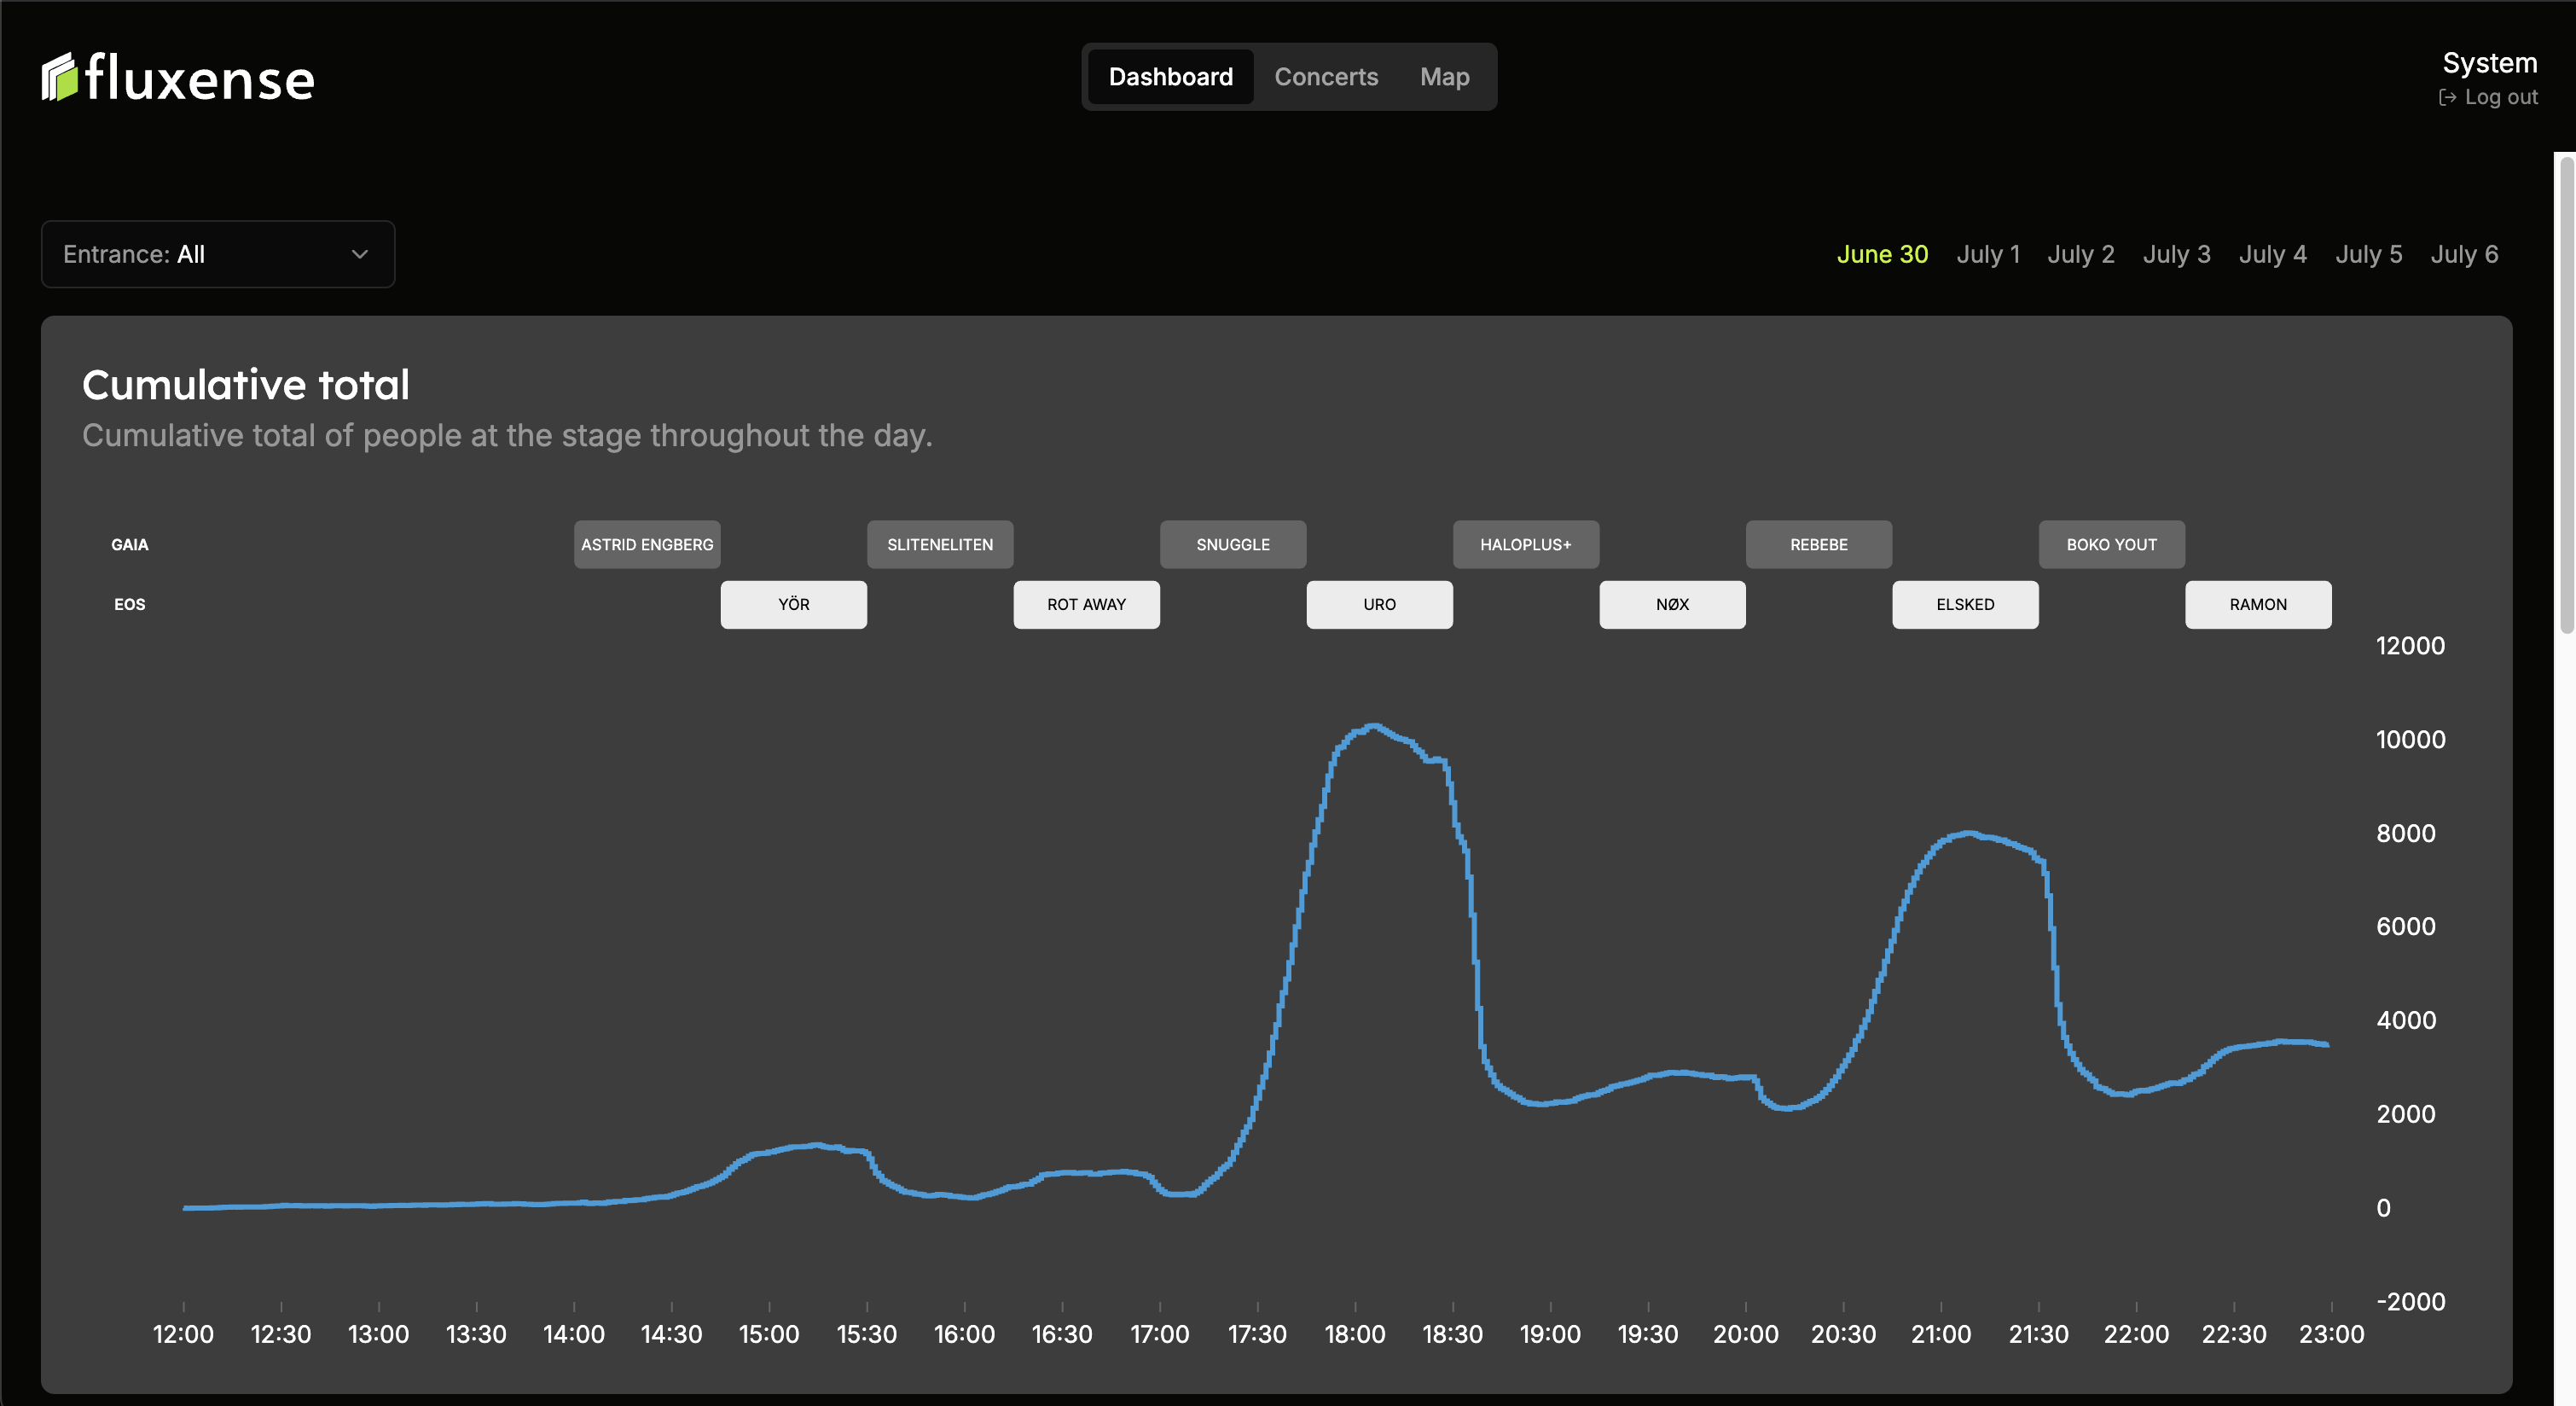
\includegraphics[width=\textwidth]{Pictures/Misc/Frontend/cum_total.png}
  \caption{The 'Dashboard' view displaying the cumulative total number of people estimated to be at the selected stage (Eos or Arena) throughout the day. An overlay along the top indicates the scheduled concert timings for the observed stage. Based on feedback requesting analysis of inter-stage flow (Appendix \ref{appendix:rf-meeting-notes}), timings for potentially influential adjacent stages (e.g., Gaia when observing Eos, or Orange stage when observing Arena) were also included.}
\end{figure}


\begin{figure}[ht]
  \centering
  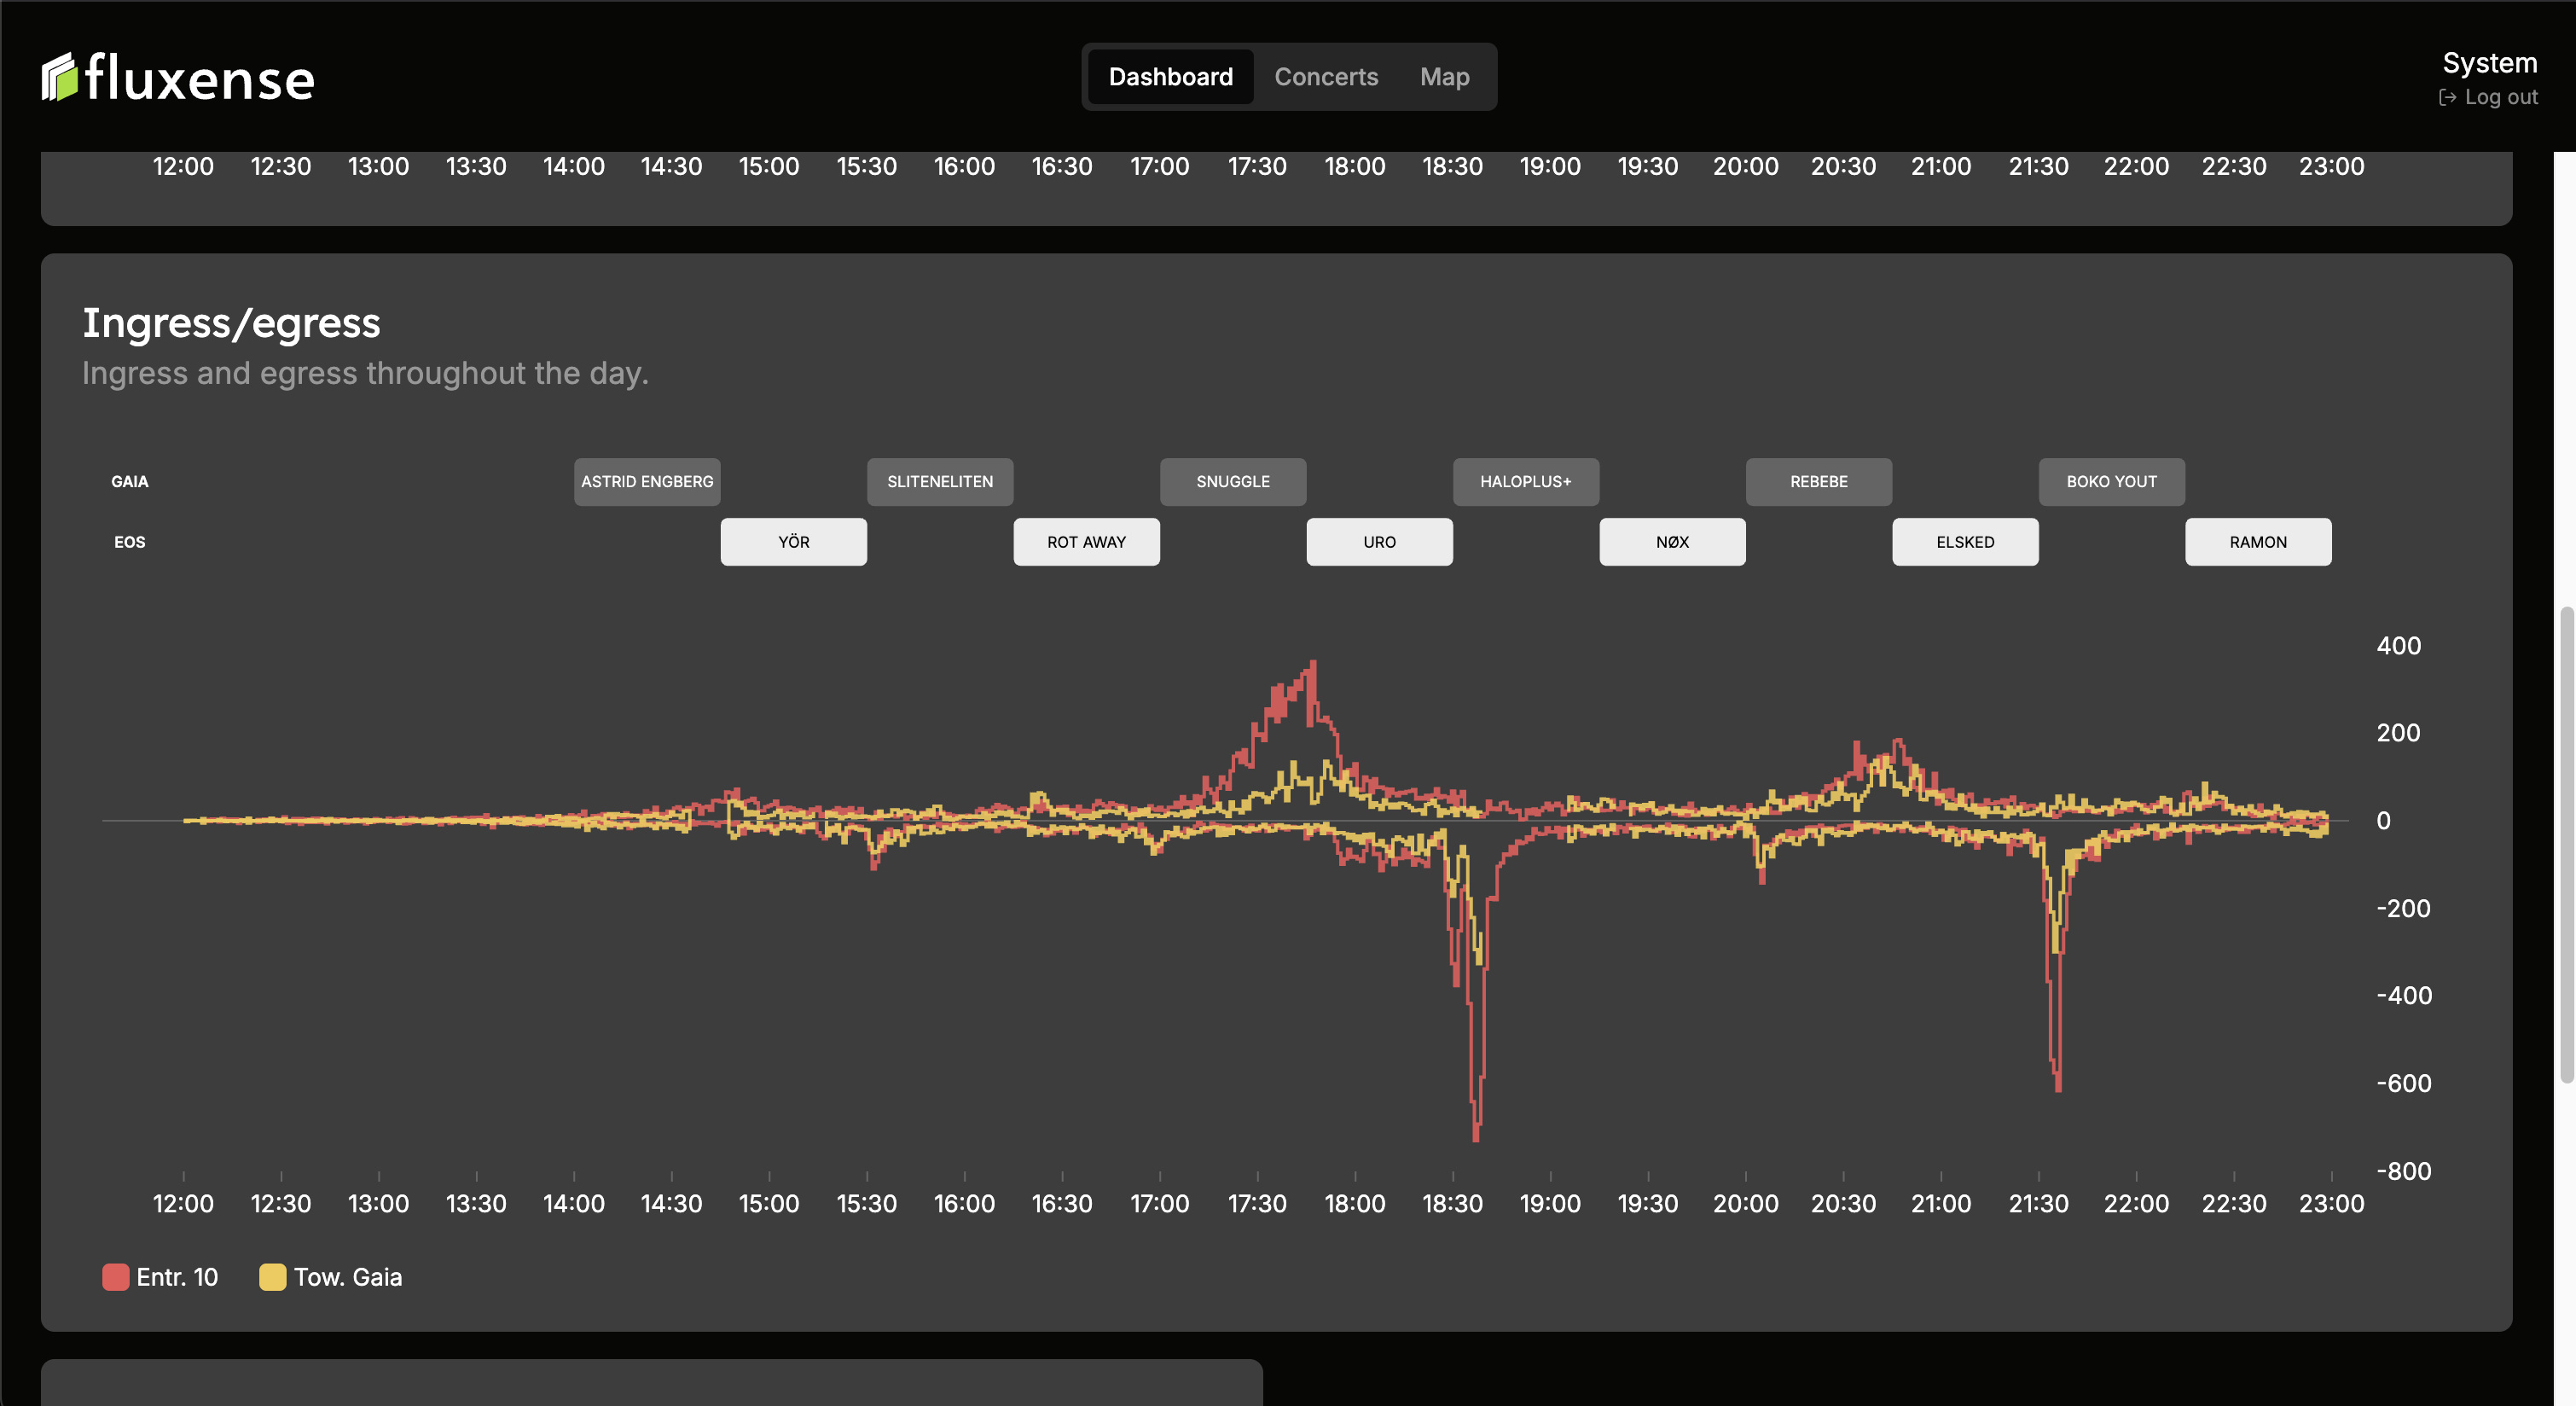
\includegraphics[width=\textwidth]{Pictures/Misc/Frontend/ingress_egress.png}
  \caption{The 'Dashboard' view showing the ingress (positive values) and egress (negative values) rates in people per minute throughout the day. Displaying data split by individual entrances (e.g., "Entr. 10", "Tow. Gaia") was implemented based on feedback requesting insight into the load of each entrance. The concert schedule overlay, including timings from relevant adjacent stages added per user feedback, is also present for context.}
\end{figure}


\begin{figure}[ht]
  \centering
  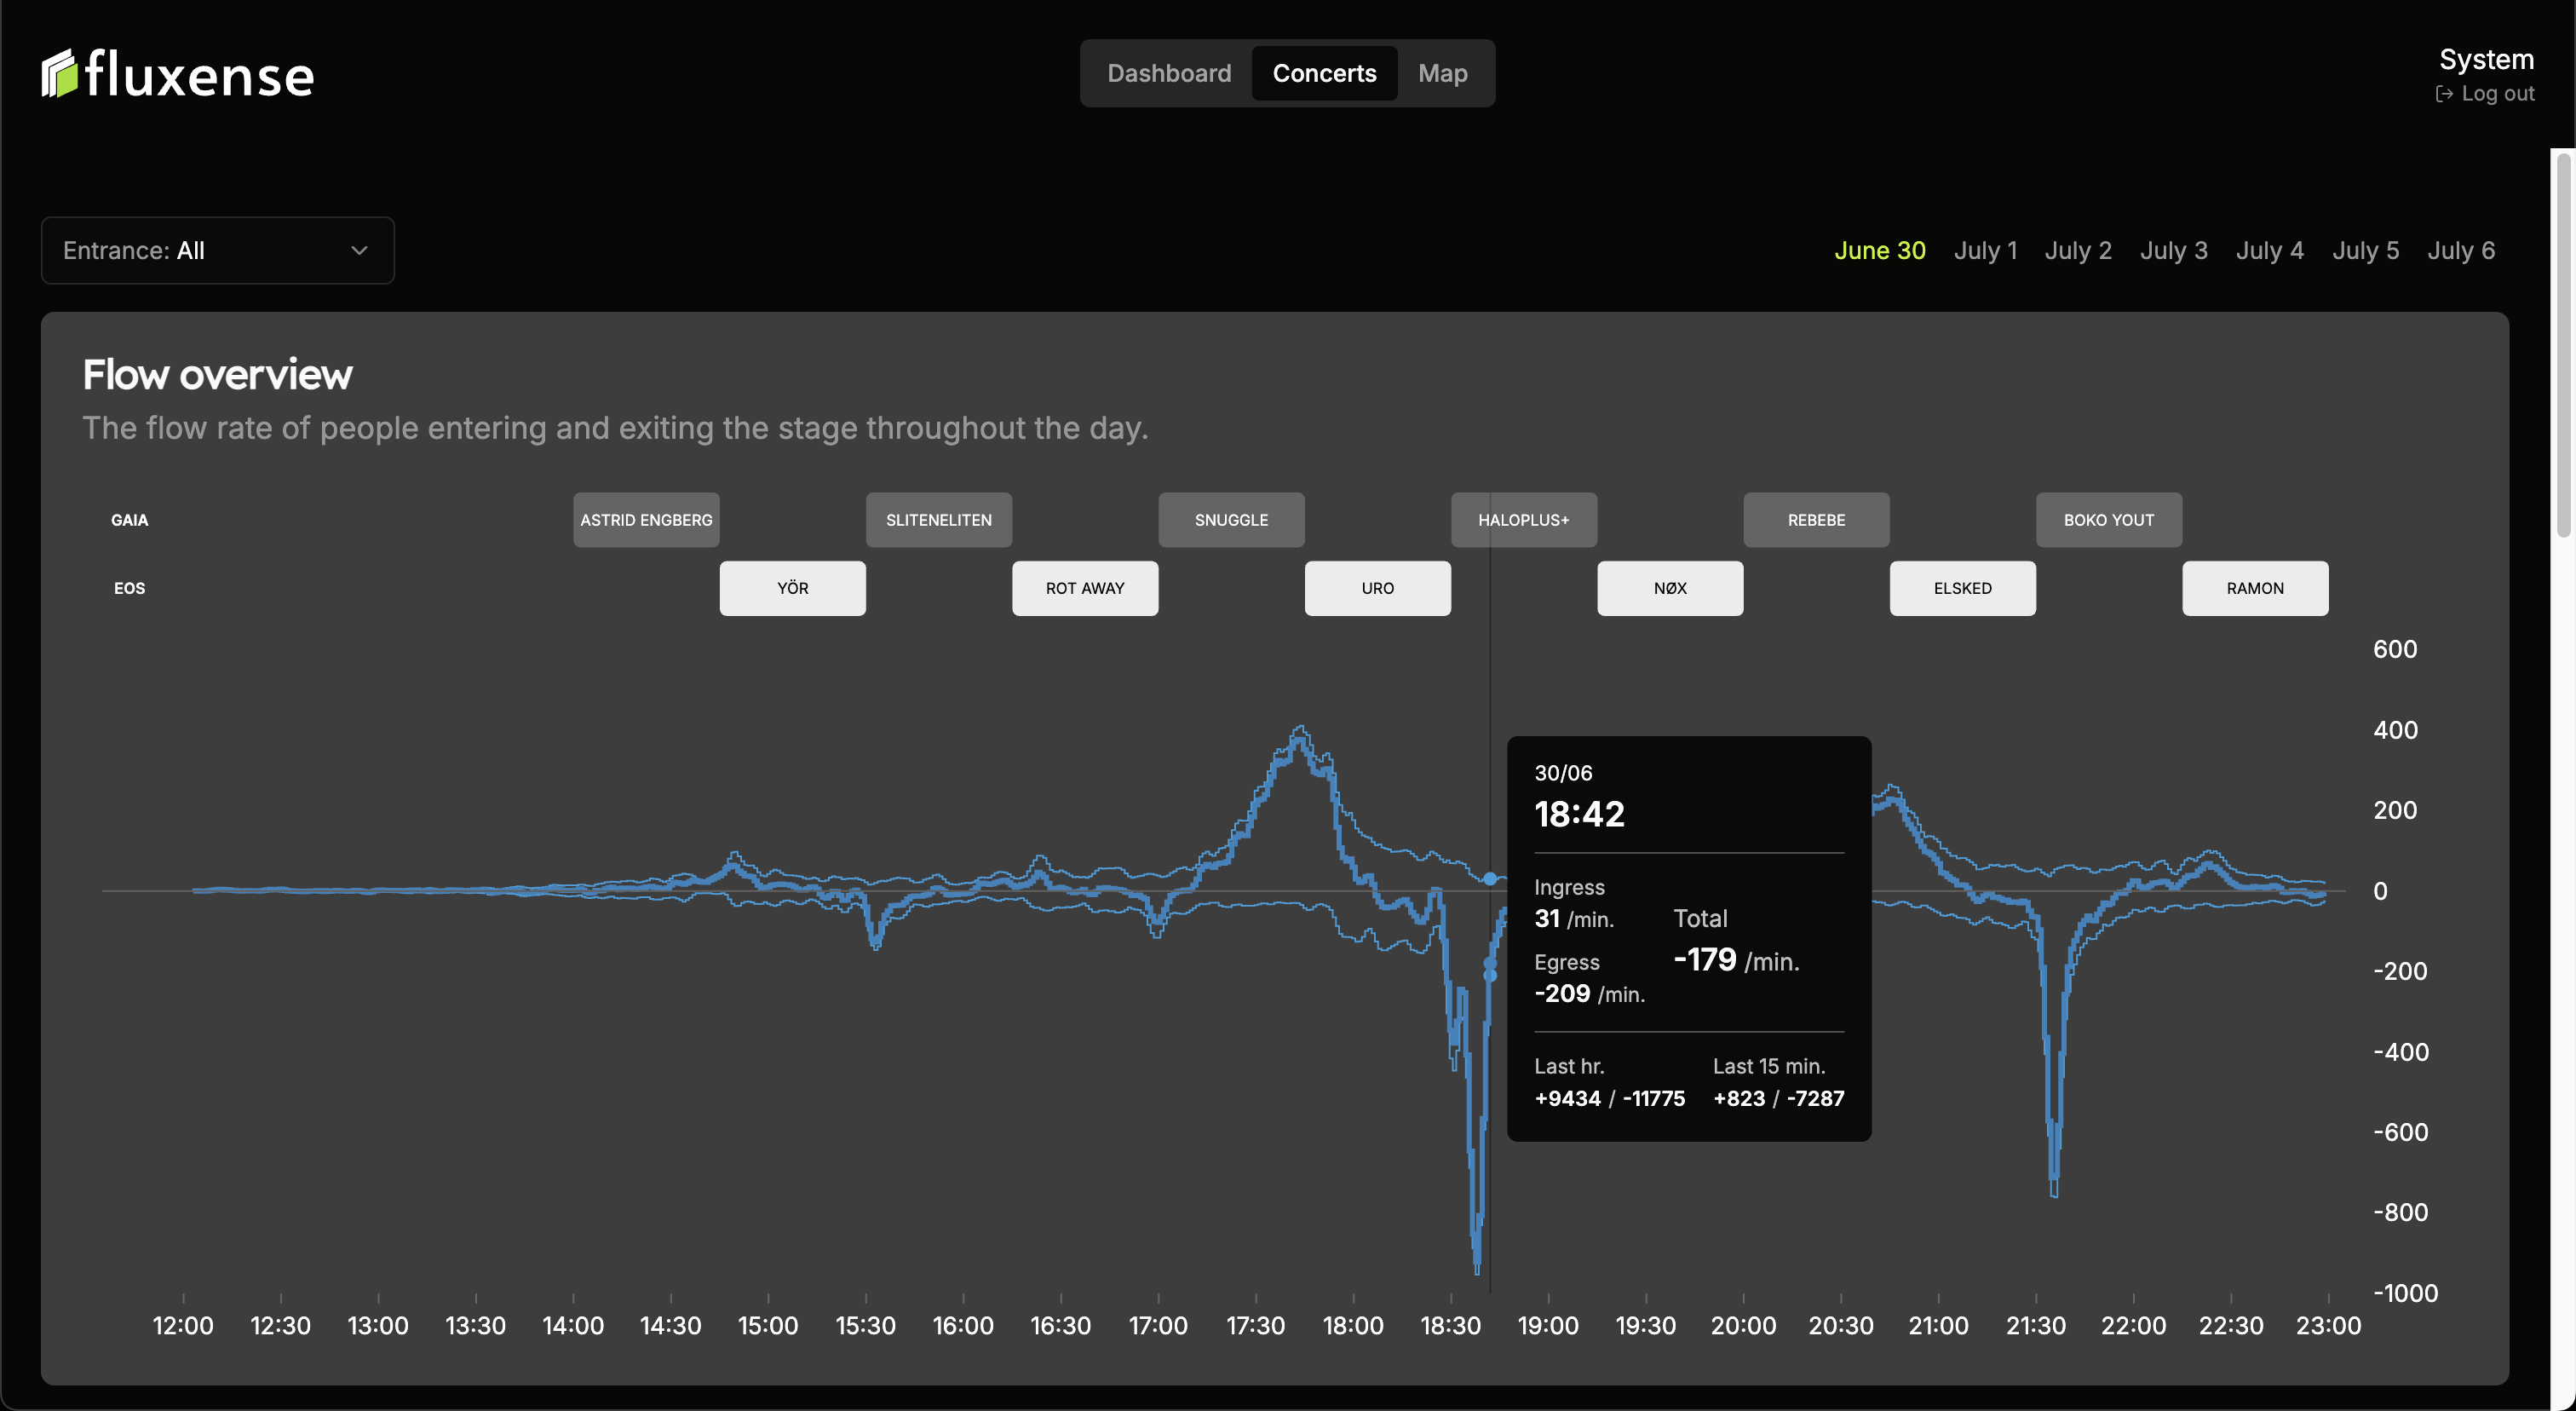
\includegraphics[width=\textwidth]{Pictures/Misc/Frontend/flow_total.png}
  \caption{The 'Concerts' view presenting the overall flow rates. It displays ingress-flow (top line), egress-flow (bottom line), and the net total flow (bold middle line). Based on feedback, flow rates are presented in people per minute for easier interpretation compared to the initial people/second unit (Appendix \ref{appendix:rf-meeting-notes}). Hovering over the chart reveals a tooltip displaying instantaneous ingress, egress, and total flow rates at a given minute, along with aggregated ingress/egress totals over the last 15 and 60 minutes, aligning with RF's requested analysis intervals. The concert schedule overlay is also present for context.}
\end{figure}

\begin{figure}[ht]
  \centering
  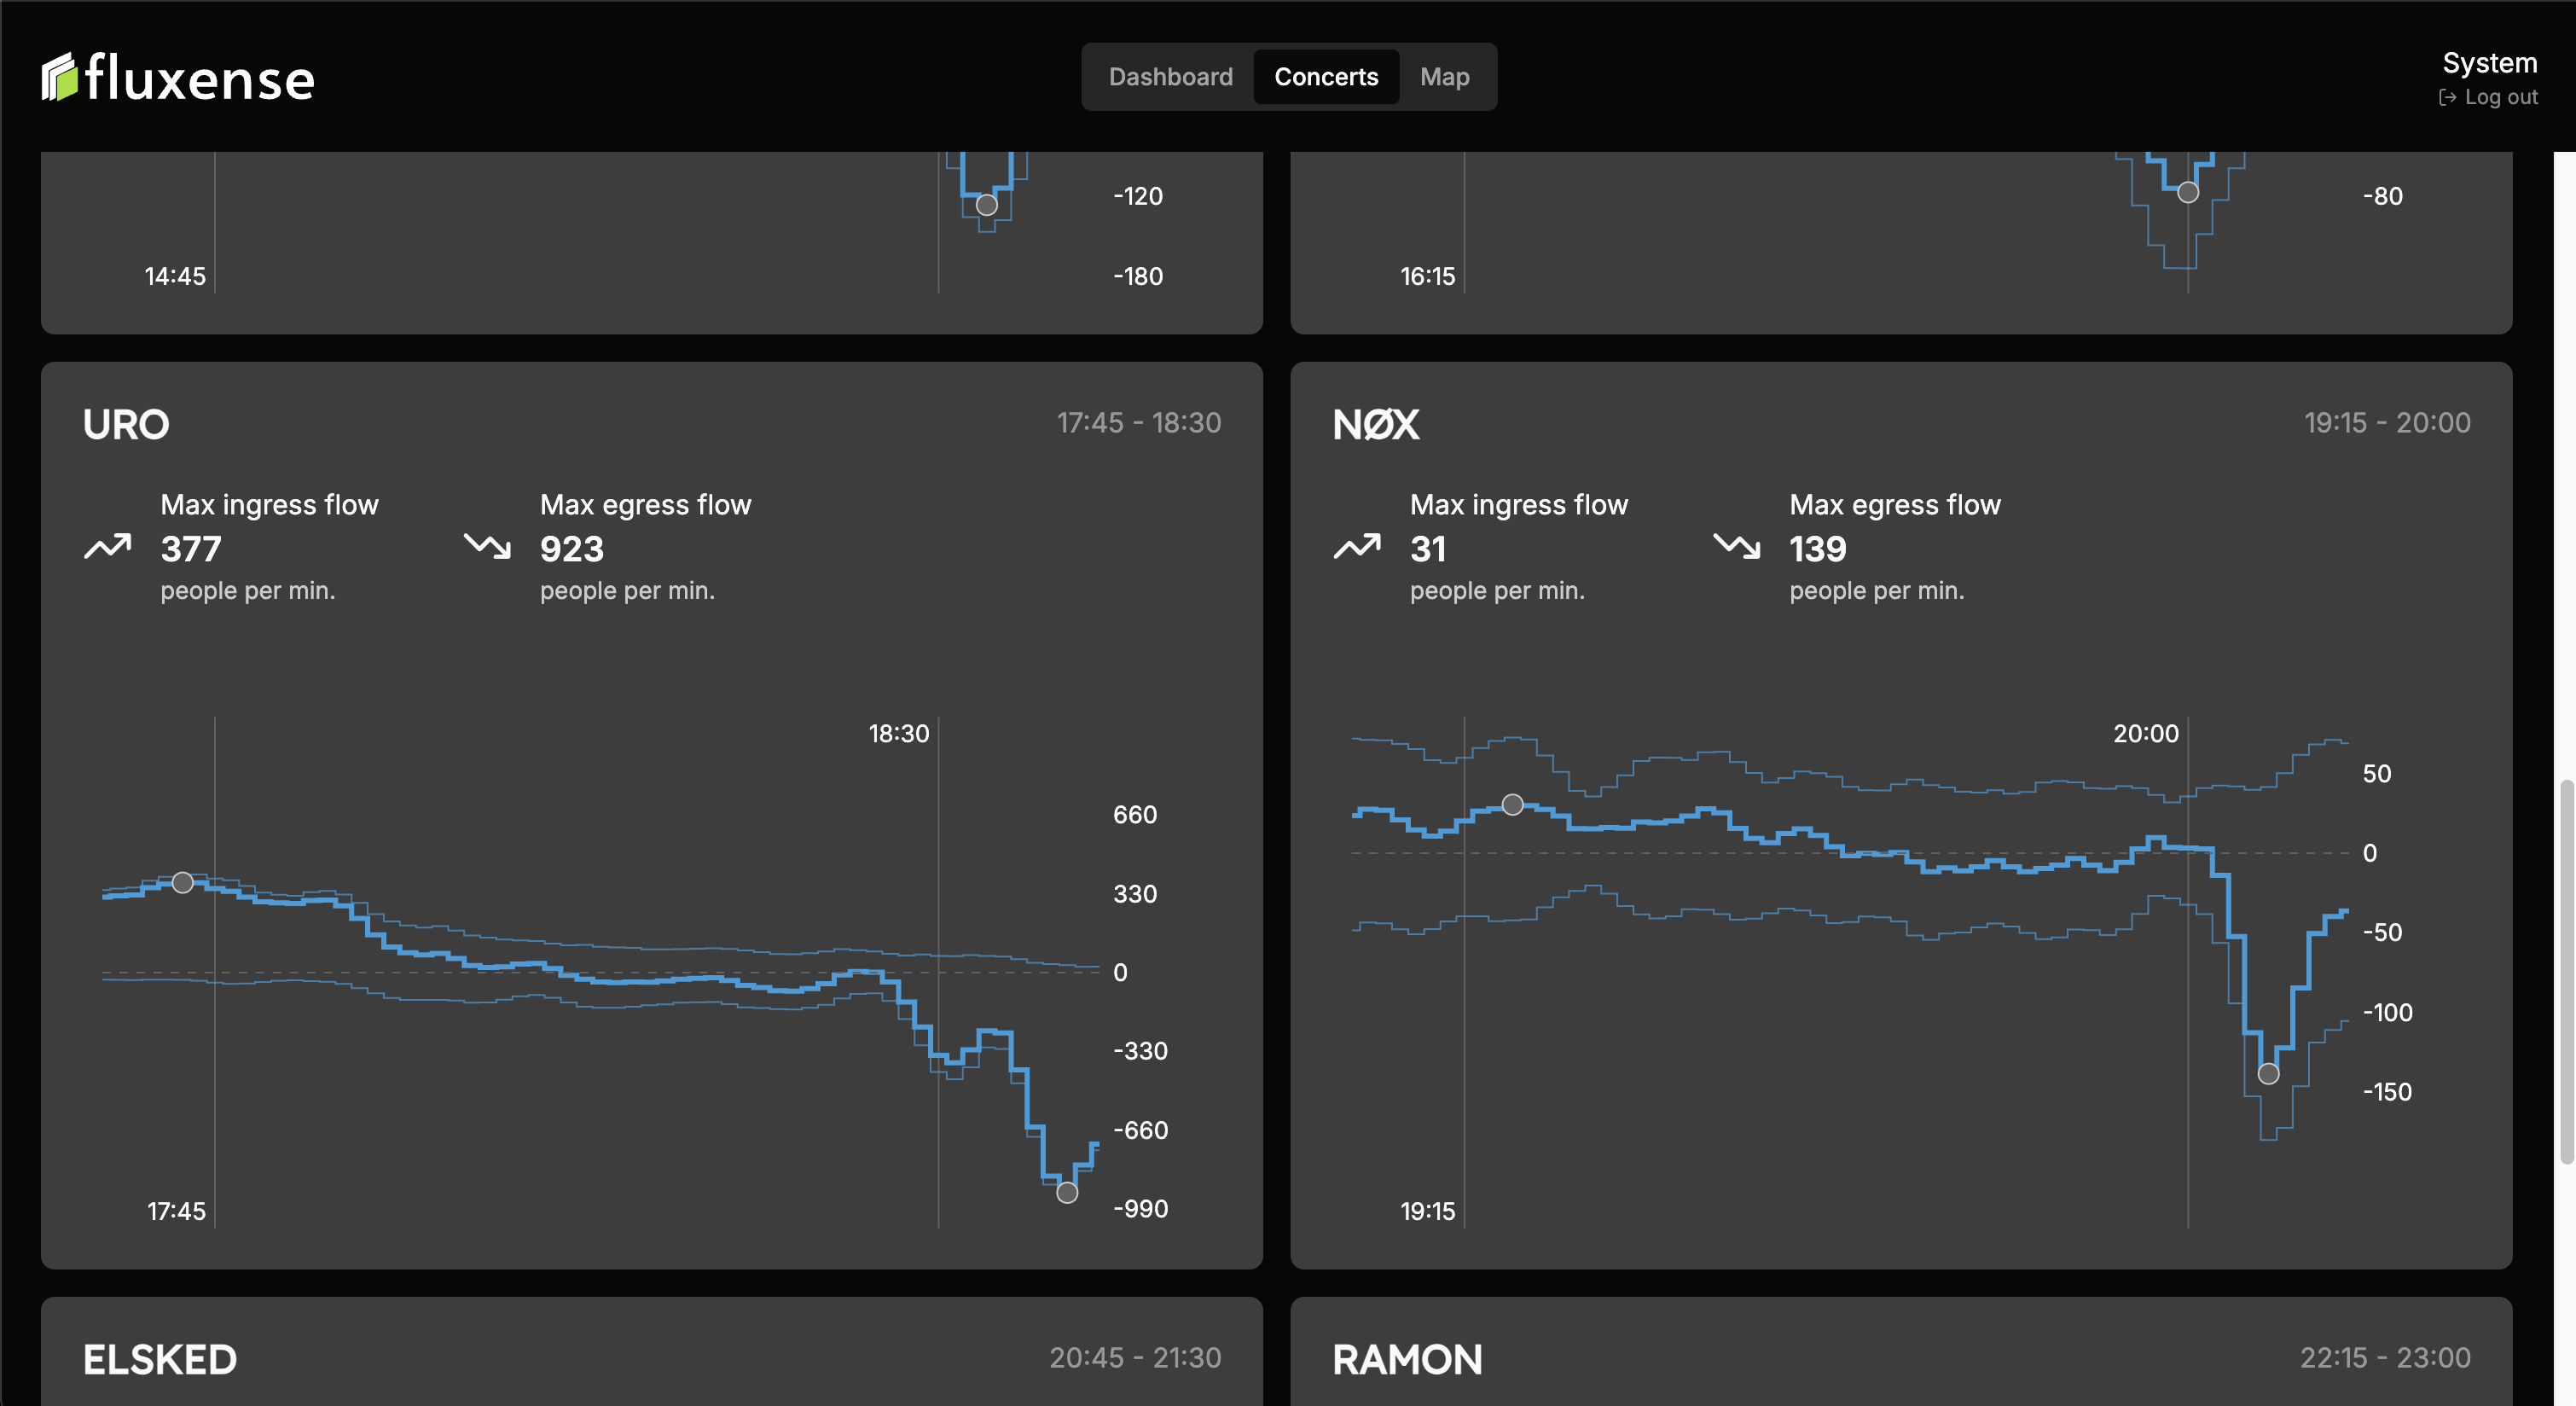
\includegraphics[width=\textwidth]{Pictures/Misc/Frontend/flow_concerts.png}
  \caption{The 'Concerts' view, with a breakdown of the flow rate data for individual concerts scheduled on the selected day. Each concert panel shows the net flow during the concert period and highlights the maximum observed ingress and egress flow rates in people per minute.}
\end{figure}

\begin{figure}[ht]
  \centering
  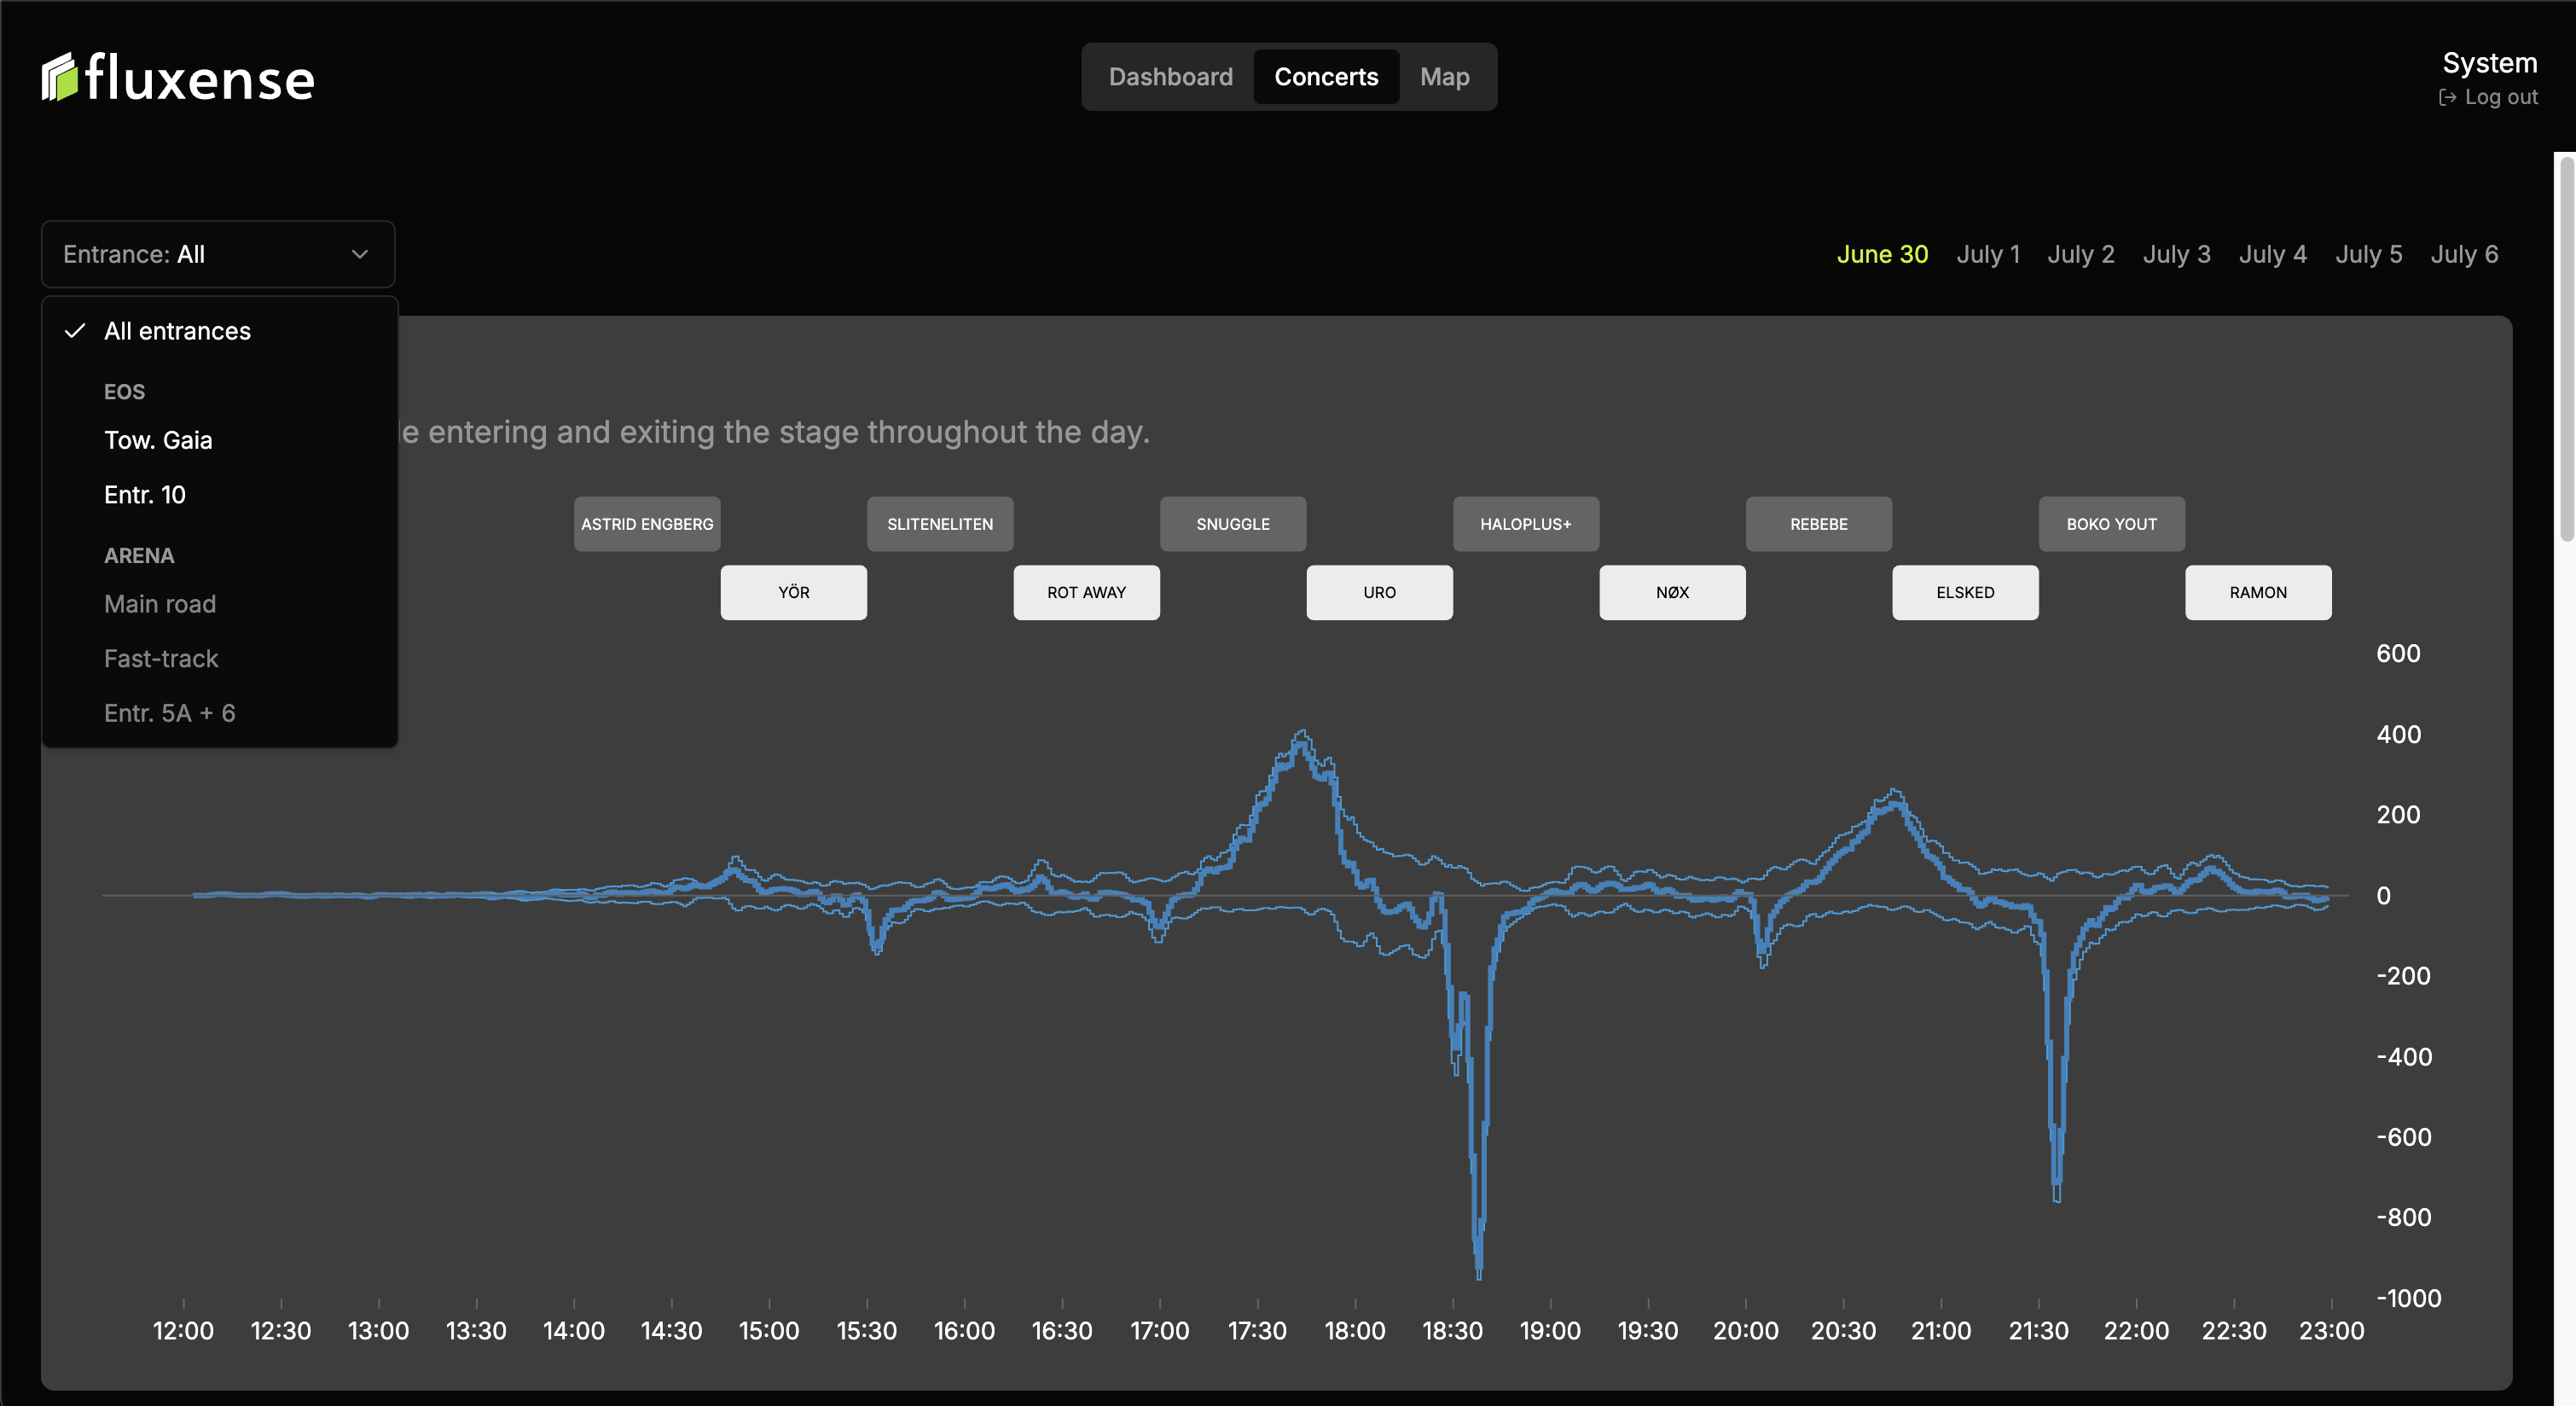
\includegraphics[width=\textwidth]{Pictures/Misc/Frontend/entrance_filter.png}
  \caption{The filtering controls available in the application, refined based on user requirements identified during feedback sessions. Users can select the date and filter the displayed data by specific entrances or view aggregated data for all entrances at a stage.}
\end{figure}

\begin{figure}[ht]
  \centering
  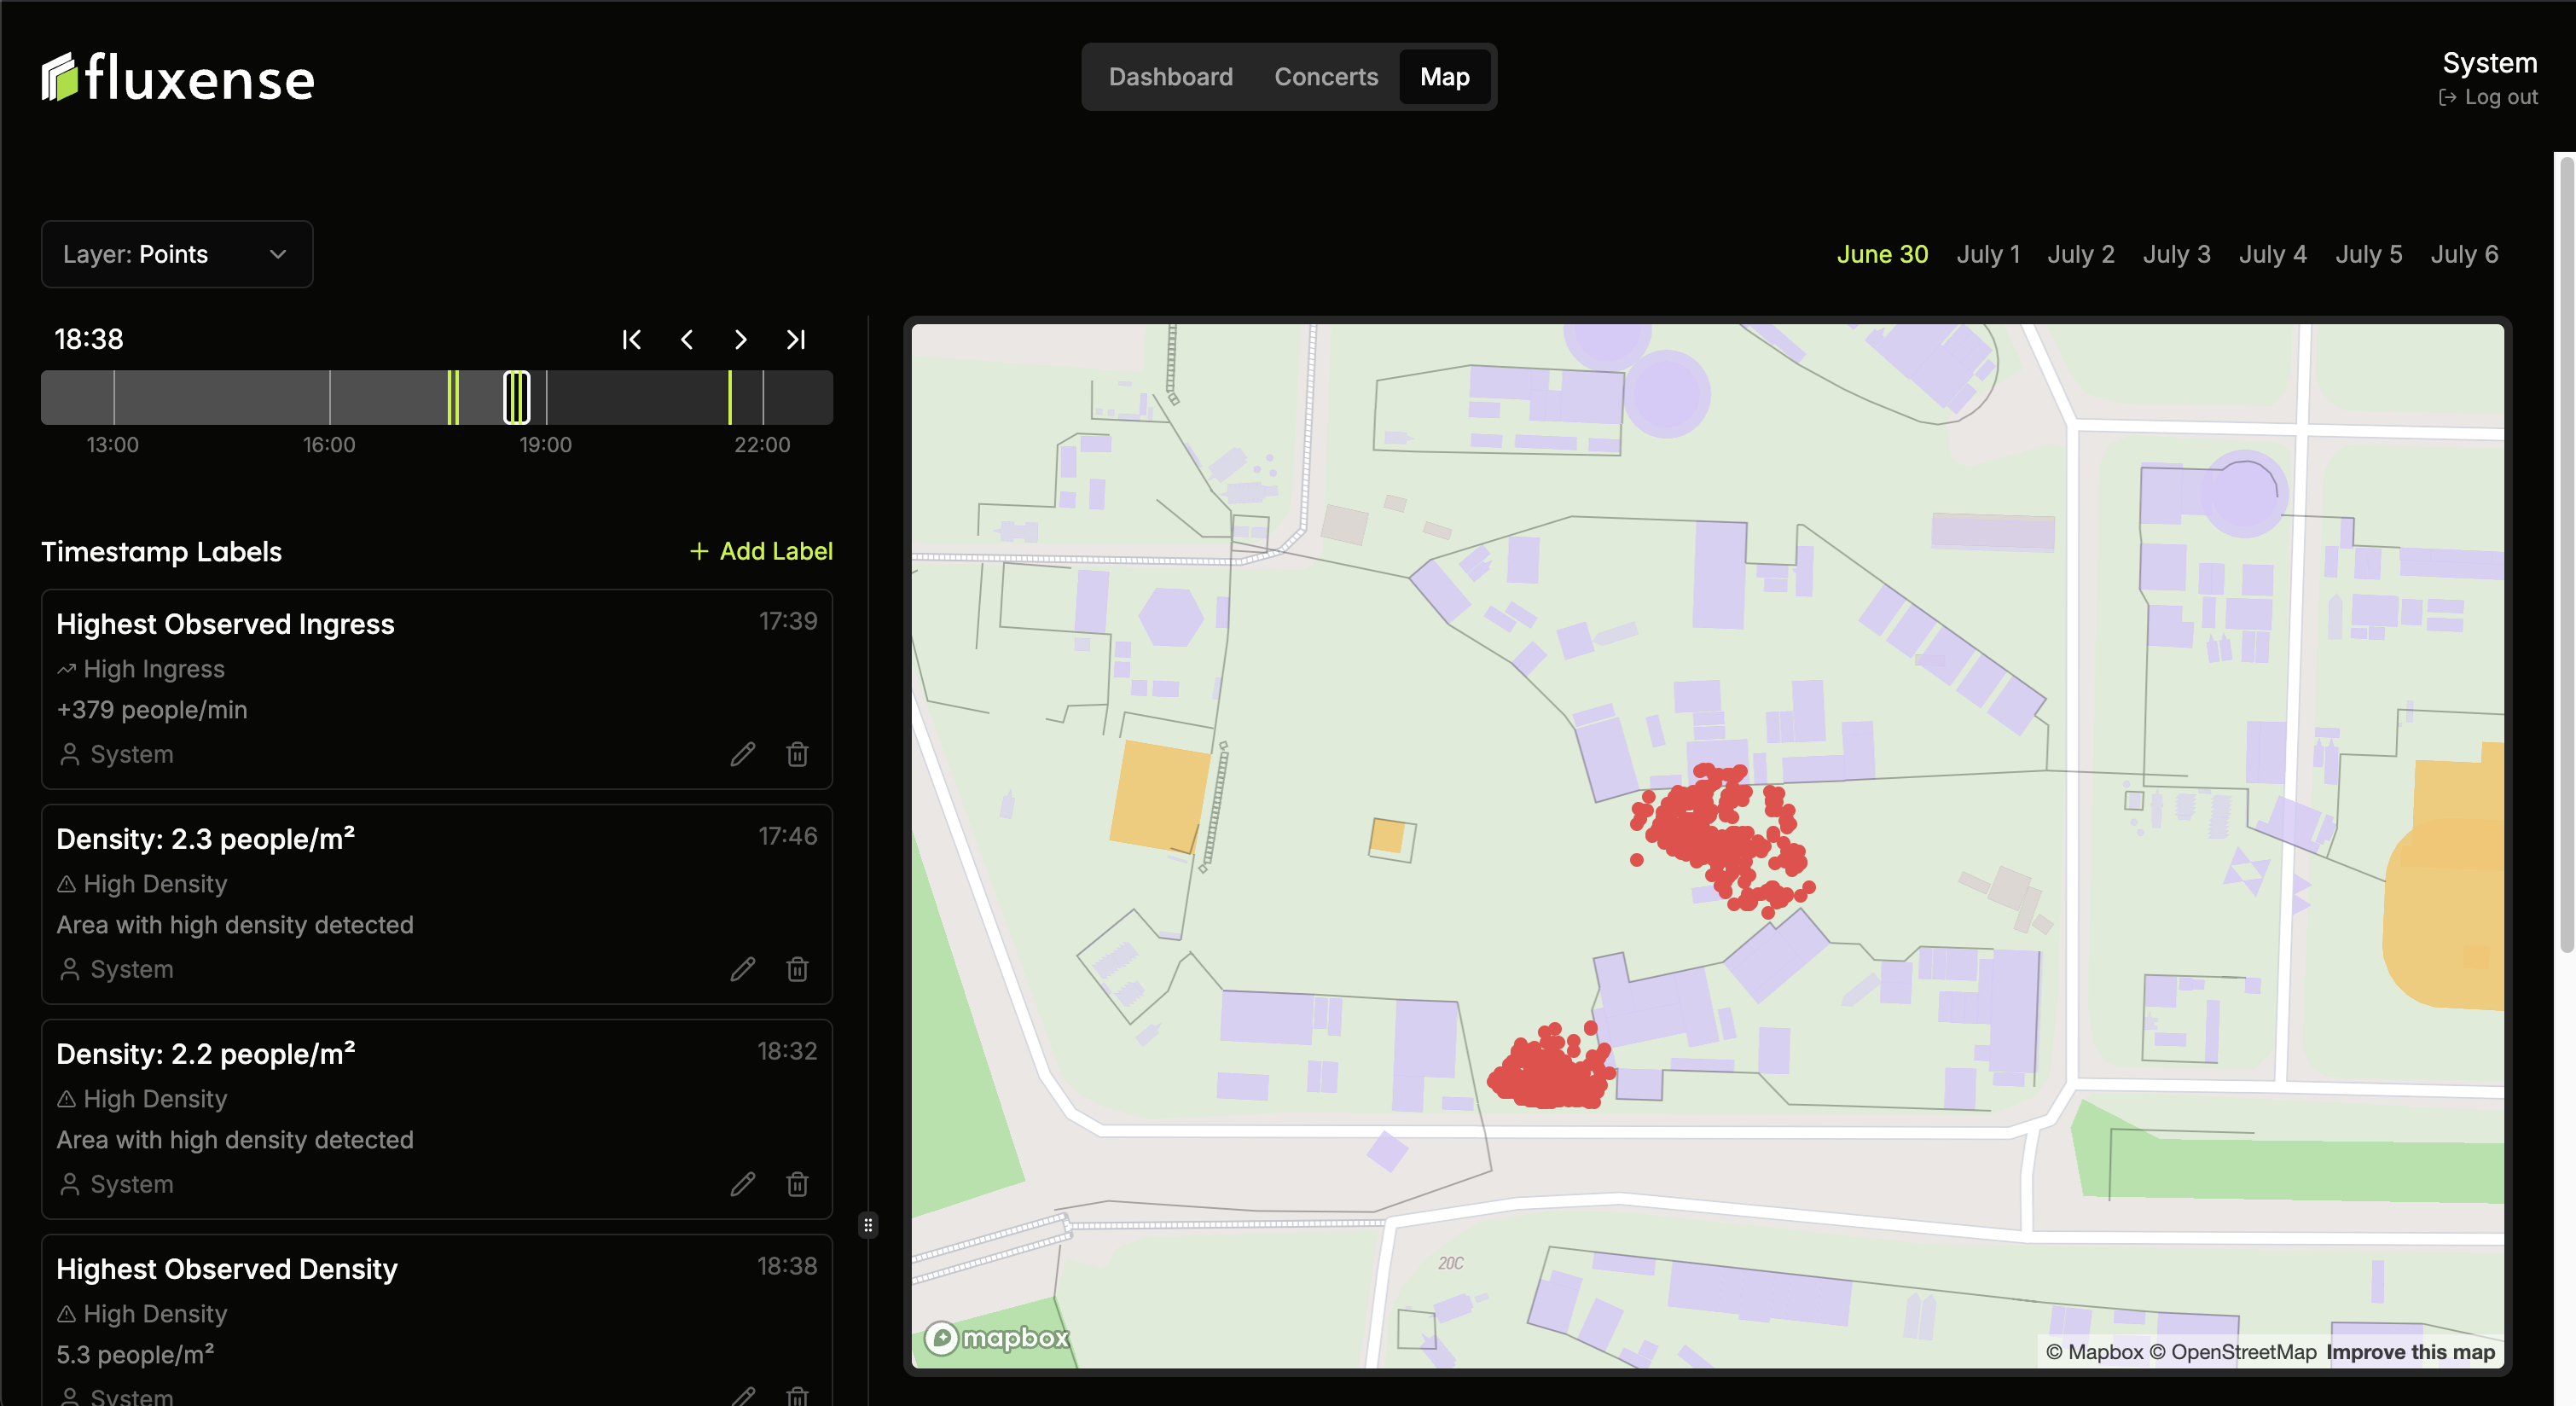
\includegraphics[width=\textwidth]{Pictures/Misc/Frontend/map_points.png}
  \caption{The 'Map' view interface elements. This includes an interactive timeline slider for navigating through the day, the 'Timestamp Labels' feature for adding user notes, and the underlying map displaying data annotations for the selected time (e.g., highest observed ingress/density). The map layer itself can be configured to show individual detections as scatter points.}
\end{figure}

\begin{figure}[ht]
  \centering
  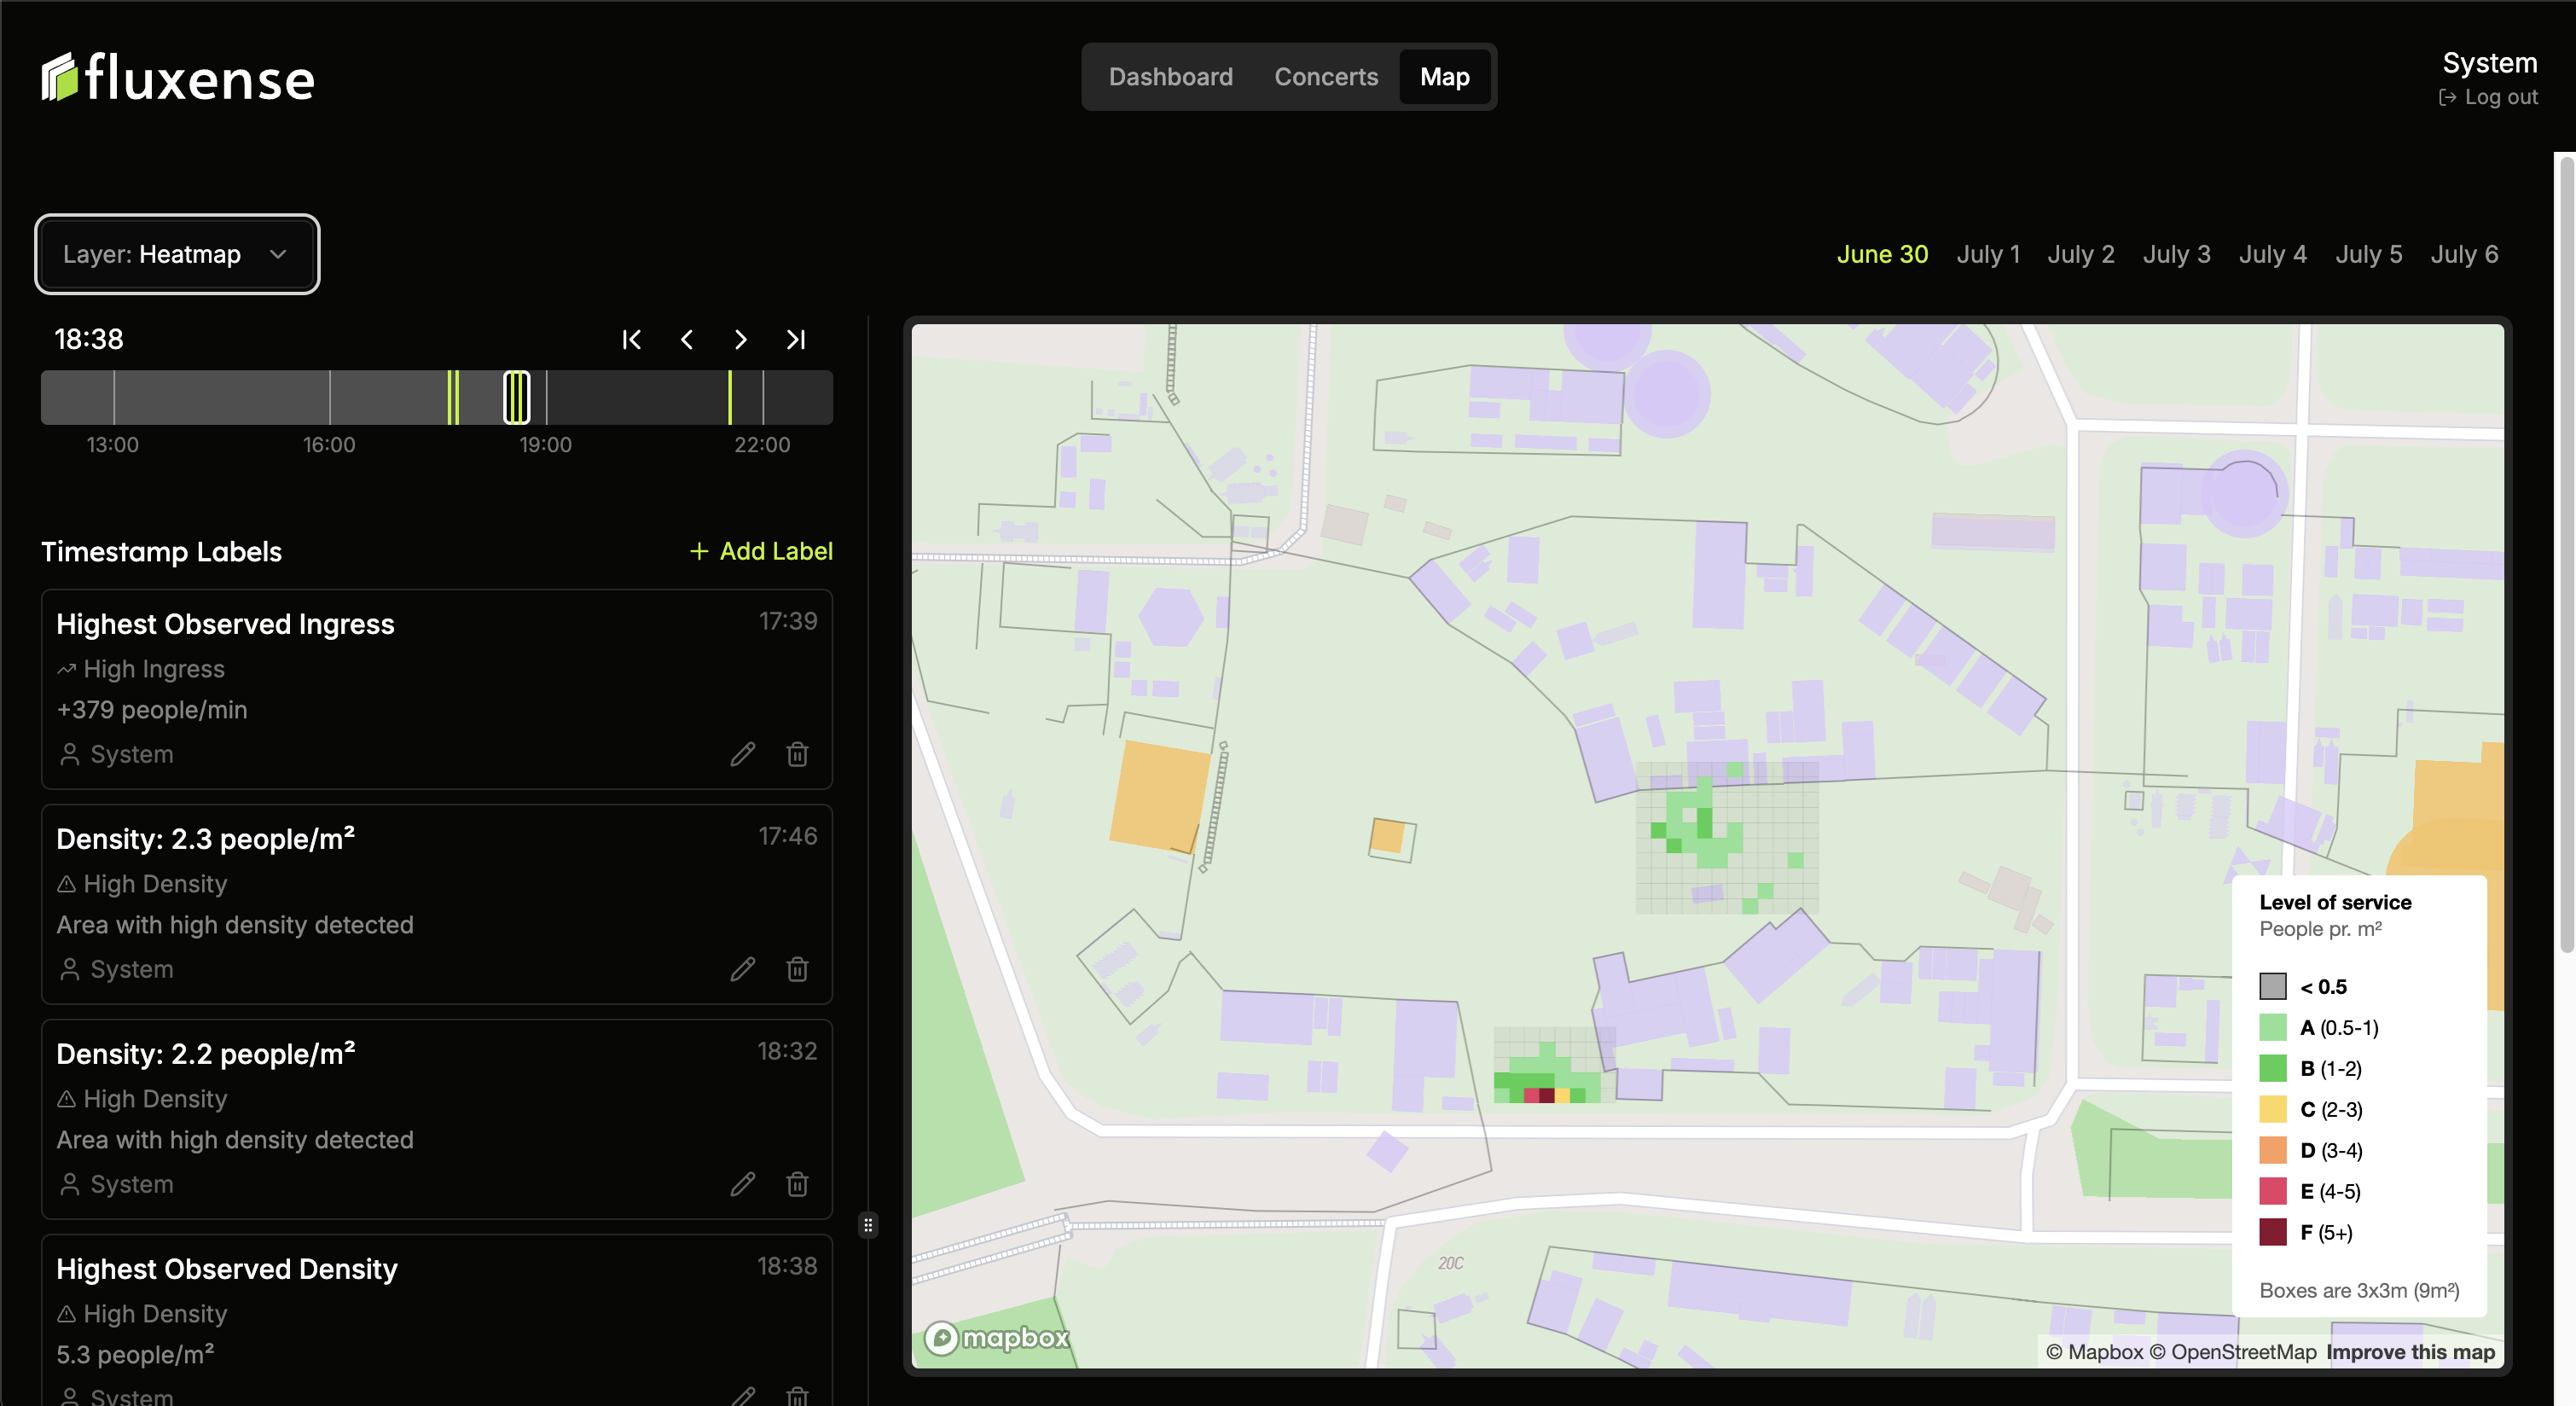
\includegraphics[width=\textwidth]{Pictures/Misc/Frontend/map_density.png}
  \caption{The 'Map' view displaying the 'Heatmap' layer. Crowd density is visualized using colored 3x3 meter grid cells. Following feedback, the color scale corresponds to Roskilde Festival's internal Levels of Service (LoS) scale (A-F), indicating people per square meter (people/m\textsuperscript{2}) to align with their existing practices.}
\end{figure}

\begin{figure}[ht]
  \centering
  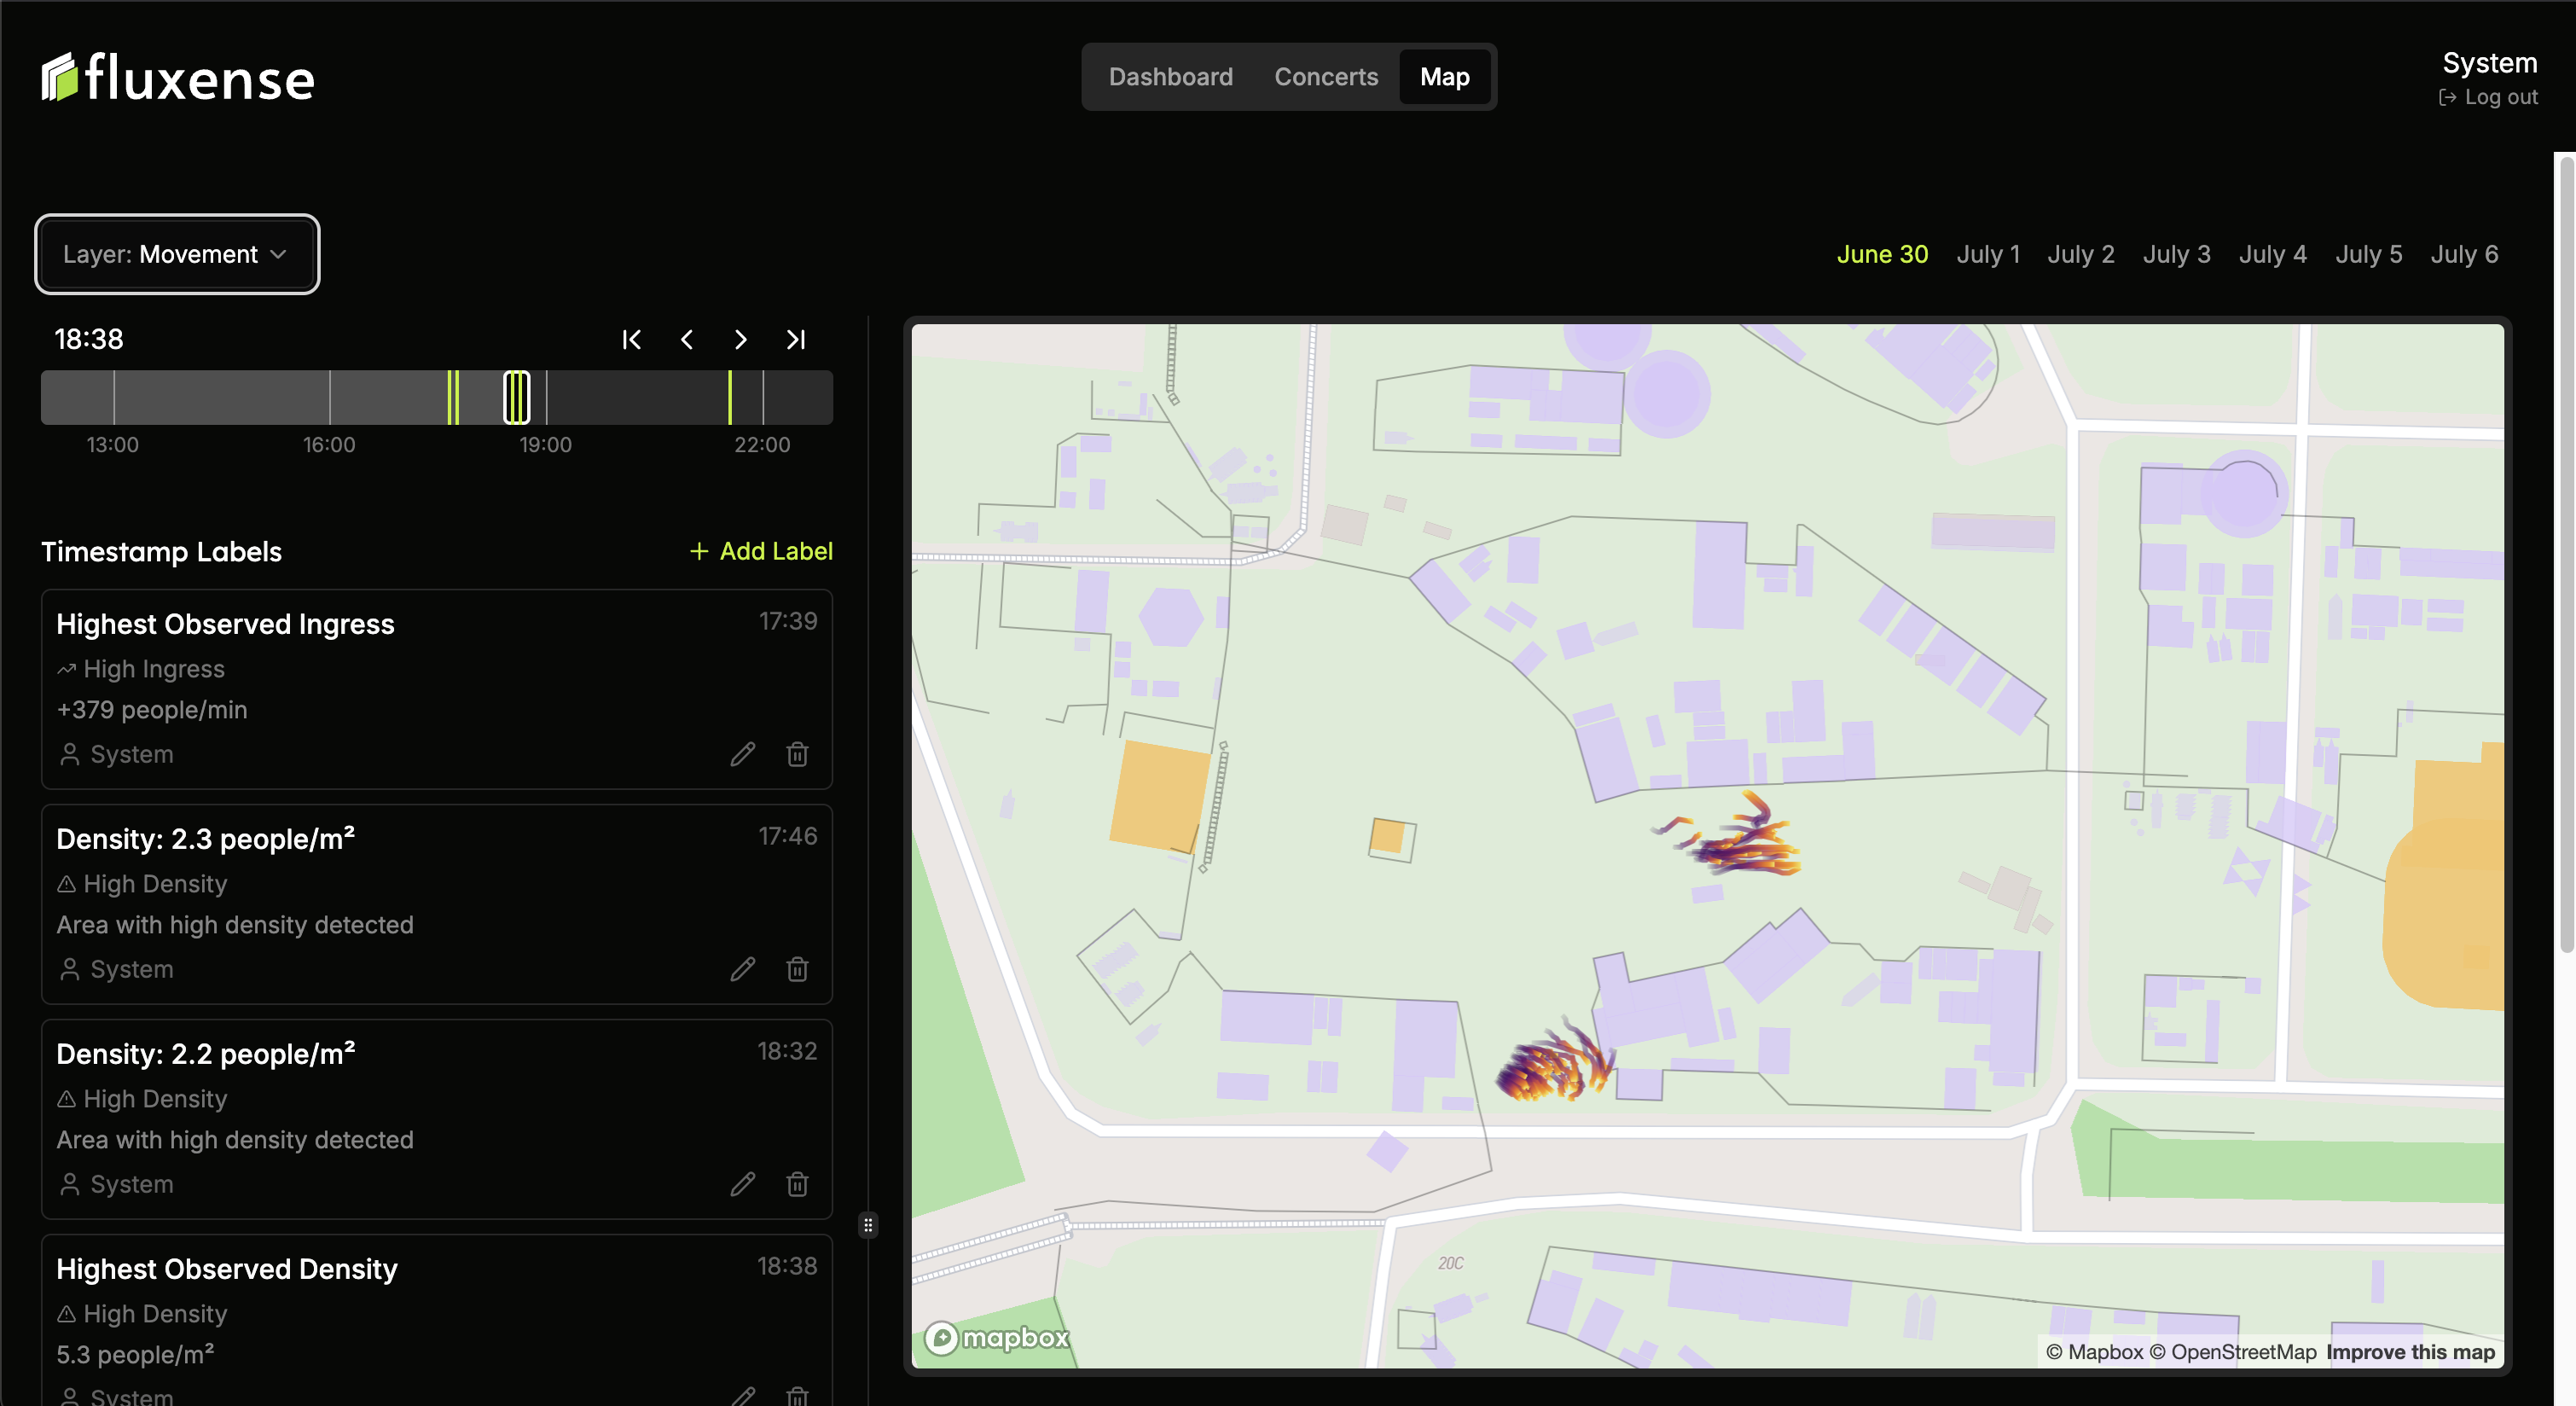
\includegraphics[width=\textwidth]{Pictures/Misc/Frontend/map_movement.png}
  \caption{The 'Map' view displaying the 'Movement' layer. Developed in response to feedback requesting visualization of movement patterns, it shows the trajectories of tracked individuals as lines on the map, with color gradients indicating the direction of movement, helping to visualize flow and origin-destination patterns.}
\end{figure}

The project successfully met its requirement specifications (Section \ref{sec:objectives}) through a combination of robust backend processing and a user-centered frontend design developed iteratively with user feedback. Core metric extraction was achieved via a pipeline utilizing computer vision for head detection and tracking, spatial mapping for real-world positioning, and dedicated algorithms to calculate key anonymized metrics like crowd density, ingress/egress flow rates at various intervals, cumulative counts, and movement patterns. An intuitive user interface was delivered as a web application featuring interactive dashboards and maps, allowing users to easily visualize these metrics through charts and geospatial displays (scatter points, heatmaps aligned with internal LoS standards, movement lines), filter data by date and location, and navigate historical data via a timeline, directly addressing usability needs confirmed in feedback sessions. Finally, compliant data handling was addressed by focusing analysis on anonymized crowd data rather than individuals, implementing secure user logins for accessing the platform, and acknowledging the need to adhere to data protection regulations like GDPR in system design.


\section{Technical performance evaluation}


\section{Business value}